\documentclass{ximera}

\newcommand{\RR}{\mathbb R}
\renewcommand{\d}{\,d}
\newcommand{\dd}[2][]{\frac{d #1}{d #2}}
\renewcommand{\l}{\ell}
\newcommand{\ddx}{\frac{d}{dx}}
\newcommand{\dfn}{\textbf}
\newcommand{\eval}[1]{\bigg[ #1 \bigg]}


\author{Jim Talamo}
\license{Creative Commons 3.0 By-bC}


\outcome{Gain practice understanding the Taylor Polynomial coefficient formula}


\begin{document}
\begin{exercise}
Recall that if a function $f(x)$ has at least $n$ derivatives at a point $x=c$, then the $n$-th order Taylor Polynomial is found by requiring that the function and its first $n$ derivatives are respectively equal to the value of the Taylor Polynomial and its first $n$ derivatives at $x=c$:

\begin{align*}
f(c) &= p_n(c) \\
f'(c) &= p_n'(c) \\
f''(c) &= p_n''(c) \\ 
& \vdots \\
f^{(n)}(c) &= p_n^{(n)}(c)
\end{align*}
or, more succinctly:

\[ f^{(k)}(c) = p_n^{(k)}(c) \textrm{ for all } k=0,1,2, \ldots , n \]

where $f^{(k)}(x)$ is notation for $\frac{d^k}{dx^k}\left[f(x)\right]$.

This lead to the requirement that:
\begin{multipleChoice}
\choice{$a_k = f^{(k)}(c) $}
\choice[correct]{$a_k = \frac{f^{(k)}(c)}{k!}$}
\choice{$f^{(k)}(c) = \frac{a_k}{k!}$}
\end{multipleChoice}

We thus take as the definition for the $n$-th order Taylor Polynomial, $p_n(x)$ centered at $x=c$ for $f(x)$:

\[
p_n(x) = a_0 +a_1(x-c)+a_2(x-c)^2+\ldots+a_n(x-c)^n
\]
where $a_k = \frac{f^{(k)}(c)}{k!}$ for $k=0,1,2, \ldots , n$.

The formula makes explicit the relationship between the coefficients of the Taylor polynomial and the derivatives of the original function.  


To gain practice understanding how the formula comes about, consider the function $f(x)=e^{2x}$ and let's consider its fifth degree Taylor polynomial at $x=0$: 

\[
p_5(x) = a_0+a_1x+a_2x^2+a_3x^3+a_4x^4+a_5x^5
\]

Suppose the goal is to find $a_3$ only and we only have the requirement that $f'''(0) = p_5'''(0)$ and not the formula.  Complete the following steps:

\begin{exercise}
First, find the derivatives of $p_5(x)$:

\begin{align*}
p_5'(x) &= a_1+\answer{2} a_2x+ \answer{3} a_3x^2+\answer{4} a_4x^3+\answer{5} a_5x^4 \\
p_5''(x) &= 2\cdot \answer{1} a_2 + 3 \cdot \answer{2} a_3x+4 \cdot \answer{3} a_4x^2+5 \cdot \answer{4} a_5x^3 \\
p_5'''(x) &= 3 \cdot 2 \cdot \answer{1} a_3+4 \cdot 3 \cdot \answer{2} a_4x+5 \cdot 4 \cdot \answer{3} a_5x^2 \\
\end{align*}

Note that 3 derivatives make all terms with powers of $x$ strictly less than 3 vanish!

\begin{exercise}
Now, evaluate $p_5'''(x)$ at $x=0$ to find:

\[ p_5'''(0) = \answer{3} ! \cdot a_3+ \answer{0} a_4+ \answer{0} a_5  \]
(Note that the coefficient for $a_3$ is specifically written as a factorial).


\begin{exercise}
this of course holds for \emph{any} polynomial of the form with which we started.  The requirement that it is a Taylor polynomial for $f(x) = e^{2x}$ means that $f'''(0) = p_5'''(0)$

One one hand, we just showed that $p_5'''(0) = 3! \cdot a_3$.

On the other, we can explicitly compute $f'''(x)$ and find that $f'''(x) = \answer{8e^{2x}}$.  Thus, $f'''(0) = \answer{8}$ and the requirement reads:

\begin{align*}
f'''(0) &= p_5'''(0) \\
\answer{8} &= 3! \cdot a_3 \\
a_3 &= \frac{8}{3!}
\end{align*}

Of course, this matches the result given by the formula $a_k = \frac{f^{(k)}(c)}{k!}$ for $k=0,1,2, \ldots , n$ because it is precisely the logic you demonstrated above that is used to derive this formula in a more general context.

\begin{exercise}
We can think of the process that we just performed as:

\begin{image}
  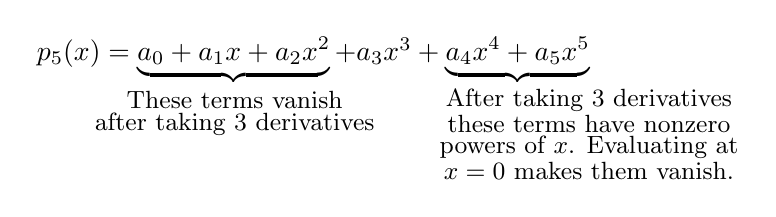
\begin{tikzpicture}
        \node at (0,0) {
          $p_5(x)= \underbrace{a_0+a_1x+a_2x^2}+a_3x^3+\underbrace{a_4x^4+a_5x^5}$};
        \node at (-1,-.5) {\small{These terms vanish}};
        \node at (-1,-.8) {\small{after taking $3$ derivatives}};
        %%
          \node at (3.5,-.5) {\small{After taking $3$ derivatives}};
          \node at (3.5,-.8) {\small{these terms have nonzero}};
            \node at (3.5,-1.1) {\small{powers  of $x$.  Evaluating at }};
             \node at (3.5,-1.4) {\small{$x=0$ makes them vanish.}};
      \end{tikzpicture}
  \end{image}

The only terms that contributes to the third derivative is the $a_3x^3$ term, since three derivatives of it will produce a constant.  By noting that $k$ derivatives of $x^k$ is $k!$, we see that this constant is precisely $\answer{3}!a_3$.

This process generalizes quite easily; indeed the formula that relates the coefficients of the Taylor polynomial to the derivatives of the original function is produced using this logic:

\begin{image}
  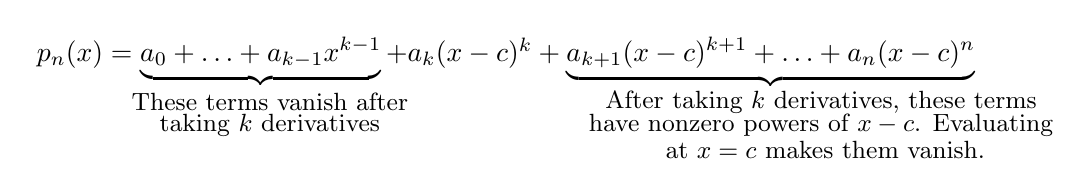
\begin{tikzpicture}
        \node at (0,0) {
          $p_n(x)= \underbrace{a_0+\ldots + a_{k-1}x^{k-1}}+a_k(x-c)^k+\underbrace{a_{k+1}(x-c)^{k+1}+\ldots+a_n(x-c)^n}$};
        \node at (-3,-.5) {\small{These terms vanish after}};
        \node at (-3,-.8) {\small{taking $k$ derivatives}};
        %%
          \node at (4,-.5) {\small{After taking $k$ derivatives, these terms}};
          \node at (4,-.8) {\small{have nonzero powers  of $x-c$.  Evaluating}};
             \node at (4,-1.1) {\small{ at  $x=c$ makes them vanish.}};
      \end{tikzpicture}
  \end{image}

The only terms that contributes to the third derivative is the $a_kx^k$ term, since three derivatives of it will produce a constant.  By noting that $k$ derivatives of $x^k$ is $k!$, we see that this constant is precisely $k!a_k$.  By equating $f^{(k)}(c)$ and $p_n^{(k)}(c)$, we find:

\[
a_k = \frac{f^{(k)}(c)}{k!}
\]


\end{exercise}

\end{exercise}
\end{exercise}
\end{exercise}
\end{exercise}
\end{document}
